\chapter{Telemanipulátor geometriája}
\label{sec:geometria}

A szakdolgozatomban elkészített telemanipulátor koncepcionális újragondolását és a kompenzációs elvárásokat az előző fejezetben bemutattam. Az elvárási szempontok figyelembevételével megterveztem a telemanipulátor geometriai vázát.

A diploma dolgozatomban bemutatásra kerülő telemanipulátor geometriájának megtervezése több féléves munka után nyerte el végső formáját. A tervezési lépéseket a kompenzáció miatt szükséges elvi felépítéstől indulva mutatom be. Végül a kinematikai felépítését és a TCP pont számításához szükséges elemzéssel zárnám a fejezetet.

%----------------------------------------------------------------------------
\section{Geometria kialakítása}
%----------------------------------------------------------------------------

A kompenzációnál megemlített paralelogramma elrendezés használata rendkívül hasznos megoldásnak bizonyult és az egyik legnagyobb fejlesztésnek tartam a szakdolgozatban dokumentált munkámhoz képest. A paralelogramma elrendezés
miatt a kábel csatornák száma az ötödik csuklóig meg kétszereződött, mivel karonként kétszer annyi elem áll rendelkezésre. Ezen túl a rendszer stabilitását is növelte az által, hogy jobban ellenáll csavaró vagy nyíró jellegű igénybe vételnek, amik a csuklókat terhelhetik. Előnyként mutatkozott ez az elrendezés akkor is amikor a számításokat végeztem, mivel a paralelogramma elrendezés azt eredményezi, hogy a minden oldala a kinematikának párhuzamos marad a vele szemköztivel. Az ötödik csuklóig így csak szinusz koszinusz számításokat és egy darab transzformációt kellett elvégeznem. Az általam elképzelt telemanipulátor kinematikai elrendezése a következő lett. A rendszer egészében $6[db]$ csuklóban mérendő szögváltozó elmozdulása alapján tudja meghatározni a TCP pontot. A elvárások alapján két darab paralelogramma kinematikai összeállítást használok és ezt követően három csuklót az end-effektorral történő mind a hat szabadsági fokon történő mozgatáshoz.

\begin{figure}[!ht]
\centering
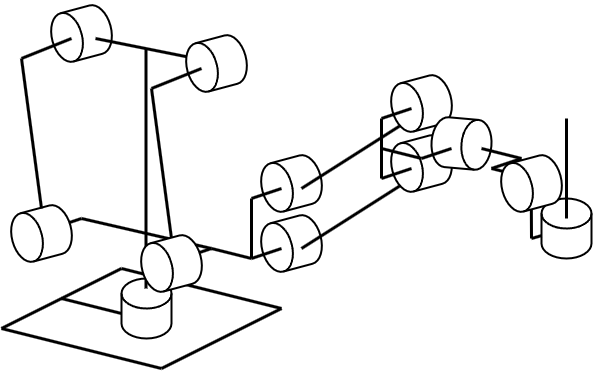
\includegraphics[width=90mm, keepaspectratio]{figures/Diagrammok/Diploma_kinematika}
\caption{Diploma munka kinematika}
\label{fig:Diploma_kinematika}
\end{figure}

A \ref{fig:Telemnanipulátor_kinematika}.ábrán láthatóan az elkészült telemanipulátor oldalról. A képen jól látható, hogy az meghatározott kinematikai lánc teljes egészében megvalósításra került. A megvalósításnál kifejezetten nagy kihívást jelentett az, hogy a karok vastagságát milyen méretűre válasszam meg. Kinematikai váz felrajzolásánál a geometriai elemek térbeli korlátjával érthető módon nem kellett foglalkozzak viszont megvalósításánál ez korlátozó tényező már nehézséget okozott.

\begin{figure}[!ht]
\centering
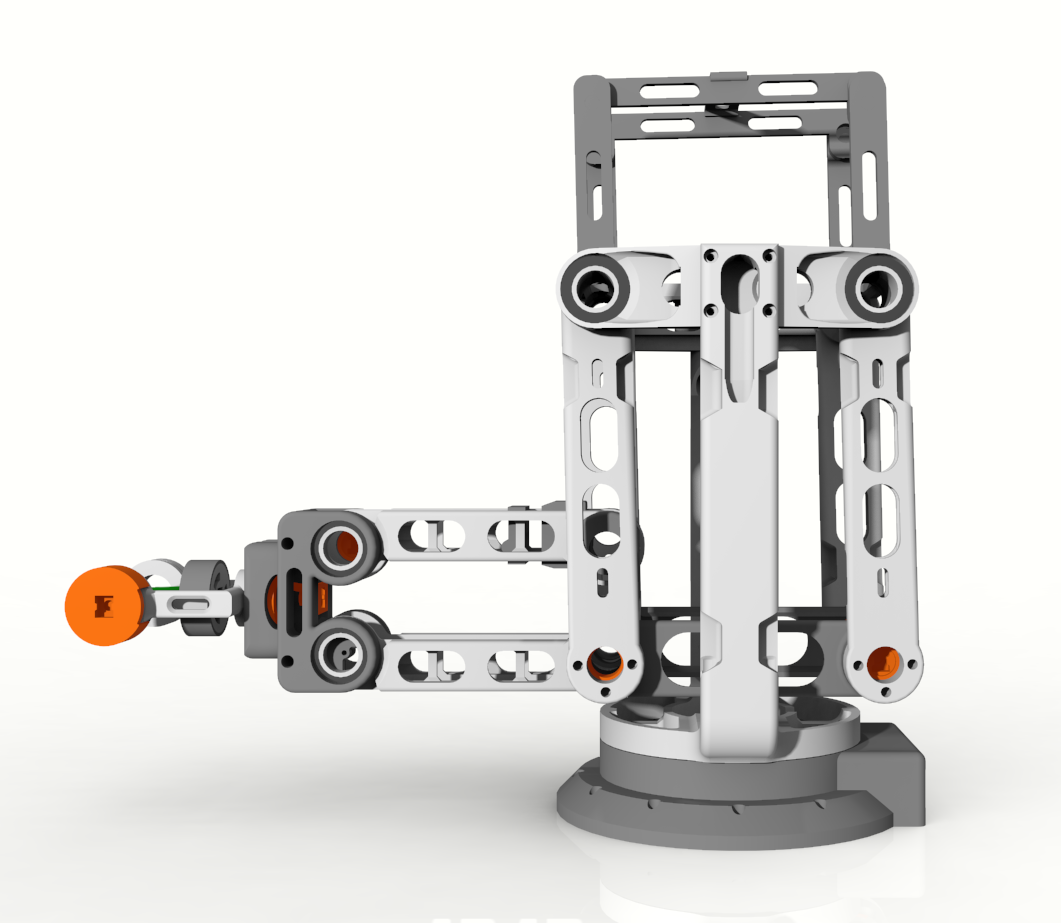
\includegraphics[width=130mm, keepaspectratio]{figures/Diploma_CAD/creo2.png}
\caption{Telemnanipulátor kinematikai elrendezésének bemutatása}
\label{fig:Telemnanipulátor_kinematika}
\end{figure}

A diploma dolgozatomban már korábban is említettem, de a továbbfejleszthetőséget nagyon fontosnak tartom. A karokat úgy terveztem meg, hogy a későbbiekben ne kelljen mindenáron az egészet kicserélni, ha új koncepciós megvalósítást készítek. A következő \ref{fig:kar}.ábrán és a \ref{fig:Csuklo_egyedul}.ábrán a második és harmadik csukló közötti kar látható, illetve a kar két végén lecsavarozható idom. Az idom illeszkedik a csapágyba illetve a kar keresztmetszetén található kábel csatornát fordítja be a tengely irányába.

\begin{figure}[!ht]
\centering
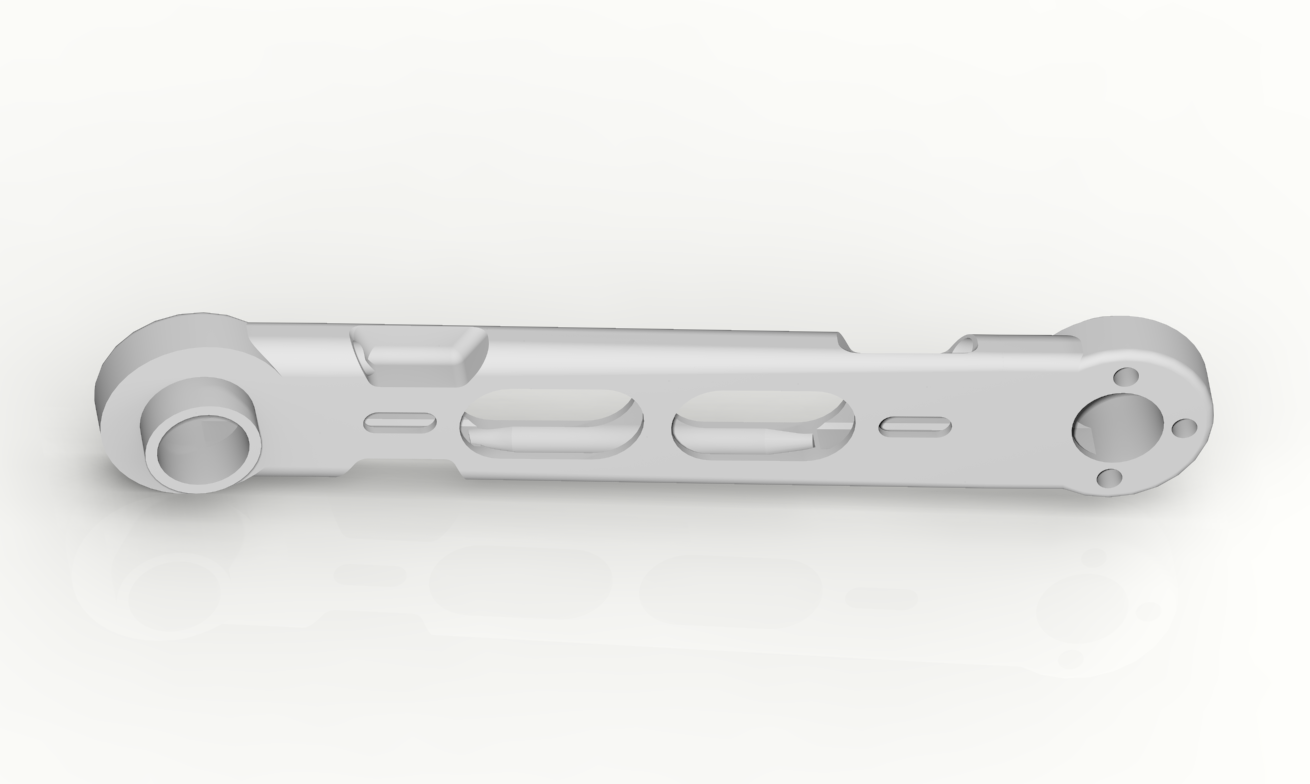
\includegraphics[width=150mm, keepaspectratio]{figures/Diploma_CAD/creo3.png}
\caption{Kar}
\label{fig:kar}
\end{figure}

Ez az idom $m4$-es csavarokkal van rögzítve a kar hosszanti testéhez. A karban réz inzerteket helyeztem így a csavart kellően feszesre meglehet húzni. A kar hosszanti elemén ovális kikönnyítéseket helyeztem el így kevesebb műanyagot használtam fel az elkészítésükhöz és könnyebbek lettek ezáltal, de a mechanikai tulajdonságaik megfelelnek az általam elvártaknak.

\begin{figure}[!ht]
\centering
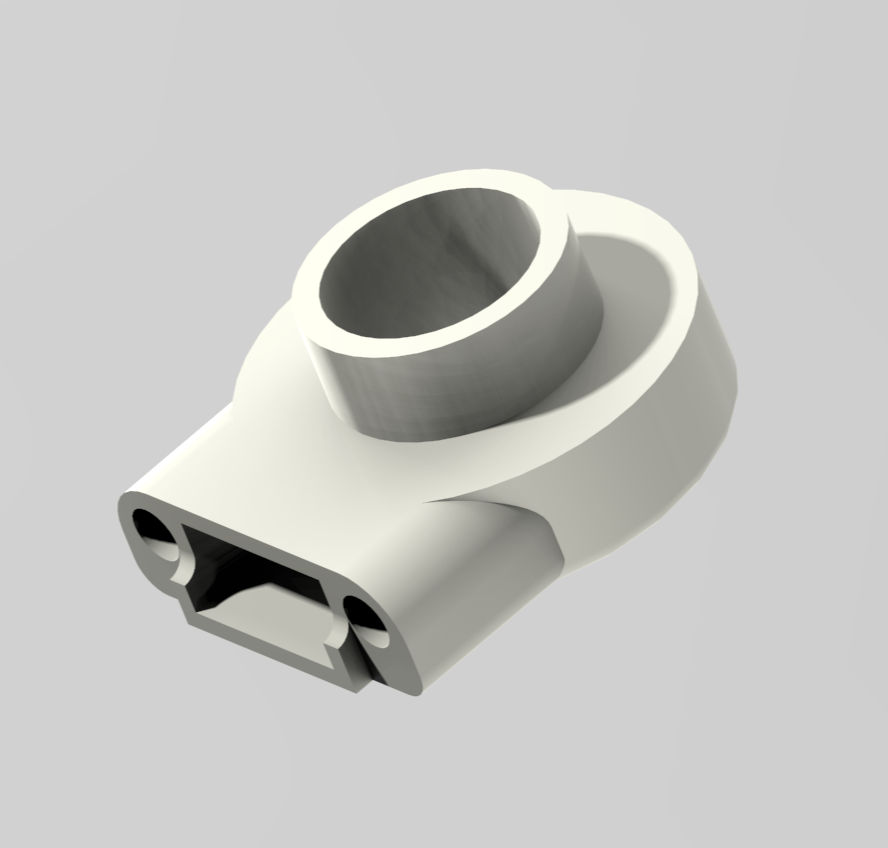
\includegraphics[width=70mm, keepaspectratio]{figures/Diploma_CAD/creo4.png}
\caption{Csuklo}
\label{fig:Csuklo_egyedul}
\end{figure}

\begin{figure}[!ht]
\centering
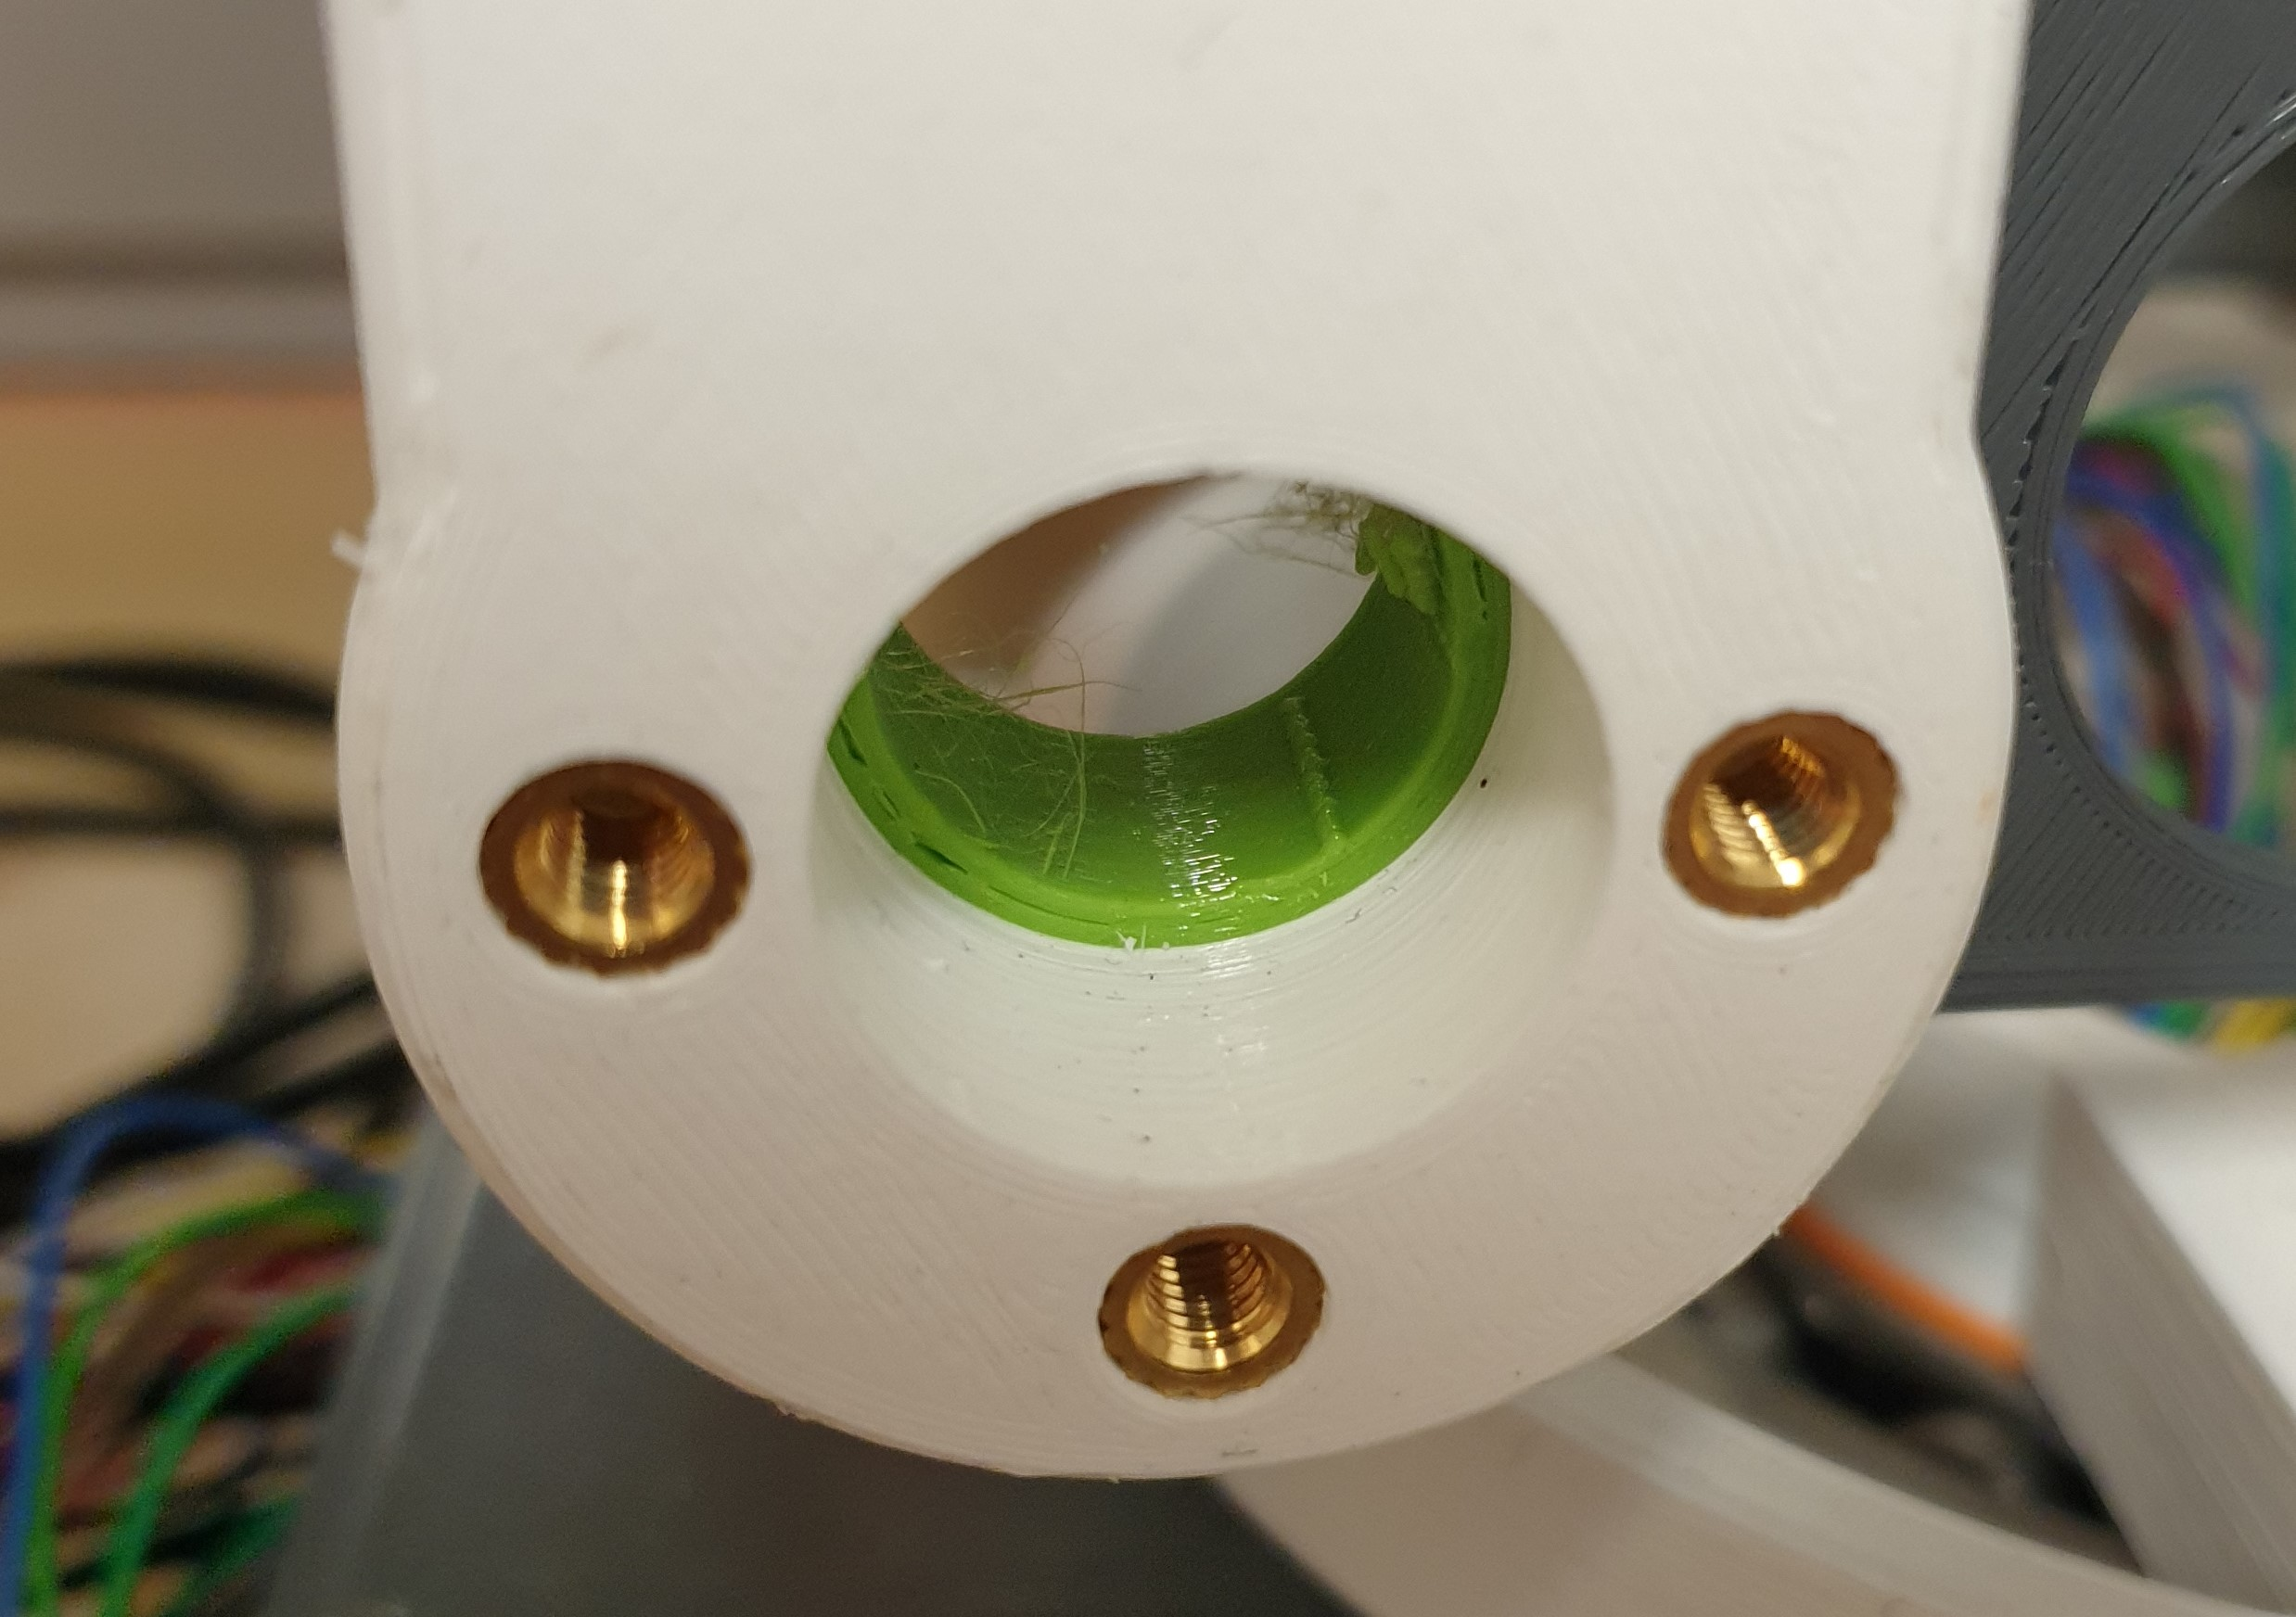
\includegraphics[width=70mm, keepaspectratio]{figures/Szumma/Inzert}
\caption{Csuklóba helyezett inzertek}
\label{fig:Csuklo_inzert}
\end{figure}

A telemanipulátor minden egyes elemének bemutatását nem tartom fontosnak, mivel minden esetben a megfelelő mennyiségű kábel elvezethetőségét, a kellően nagy méretet és a optimális anyag felhasználást tartottam szem előtt. A következőképen a látható a teljes telemanipulátor. Az end-effektorról még ejtek párszót, de előtte a geometriai méreteket ismertetném és ezzel érzékelhetővé válik a szakdolgozatomban és az itt bemutatásra kerülő telemanipulátor méretbeli különbsége. A következő táblázat gyűjti össze a geometriai paramétereket.

\begin{table}[!ht]
\centering
\begin{tabular}{ |c|c|c| }
 \hline
 Kar sorszám & Karhossza milliméterben  \\
 \hline
 Első kar & $290[mm]$  \\
 \hline
 Második kar & $200[mm]$  \\
 \hline
 Harmadik kar & $150[mm]$  \\
 \hline
 Negyedik kar & $87.5[mm]$  \\
 \hline
 Ötödik kar & $48[mm]$  \\
 \hline
 Hatodik kar & $30[mm]$  \\
\hline
\end{tabular}
\caption{Telemanipulátor karjainak méretét megadó táblázat}
\label{table:merettabla}
\end{table}

A következő képen a teljes telemanipulátor tekinthető meg.

\begin{figure}[!ht]
\centering
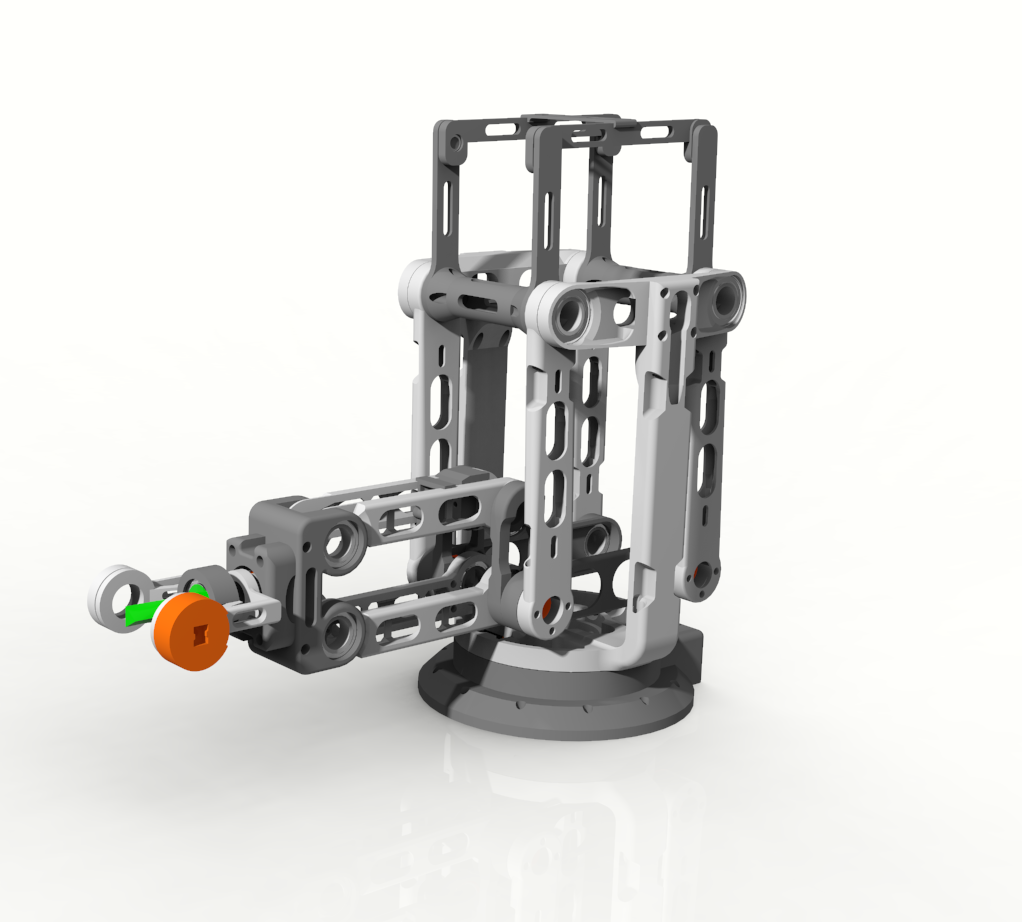
\includegraphics[width=120mm, keepaspectratio]{figures/Diploma_CAD/creo1.png}
\caption{Teljesen megtervezett telemanipulátor}
\label{fig:Telemnanipulátor}
\end{figure}

\subsection{Diplomamunkámban használt end-effektor}

A telemanipulátort úgy terveztem meg, hogy az ötödik csukló végén egy platform van, amire tetszőleges geometriát lehet csatlakoztatni. A vezeték csatlakozási lehetőségeket is biztosítottam a szenzoroknak, amivel szinte bármilyen felszenzorozott eszköz könnyen át lehet vezetni a telemanipulátor kábel csatornáin. Az így elkészített platform szinte korlátlan lehetőséget biztosít arra, hogy milyen célra használjuk fel az eszközt továbbiakban.

A telemanipulátor negyedik és ötödik csuklója közti karon található a rugós tömegkompenzációs rendszer. Ez a mechanika úgy van kialakítva, hogy egy menetes orsóval a rugó feszességét lehet állítani. Ezzel a megoldással attól függően, hogy az end-effektornak mekkora a súlya, a tömegkompenzációs rendszerben a rugó erőt lehet növelni vagy csökkenteni.

\begin{figure}[!ht]
\centering
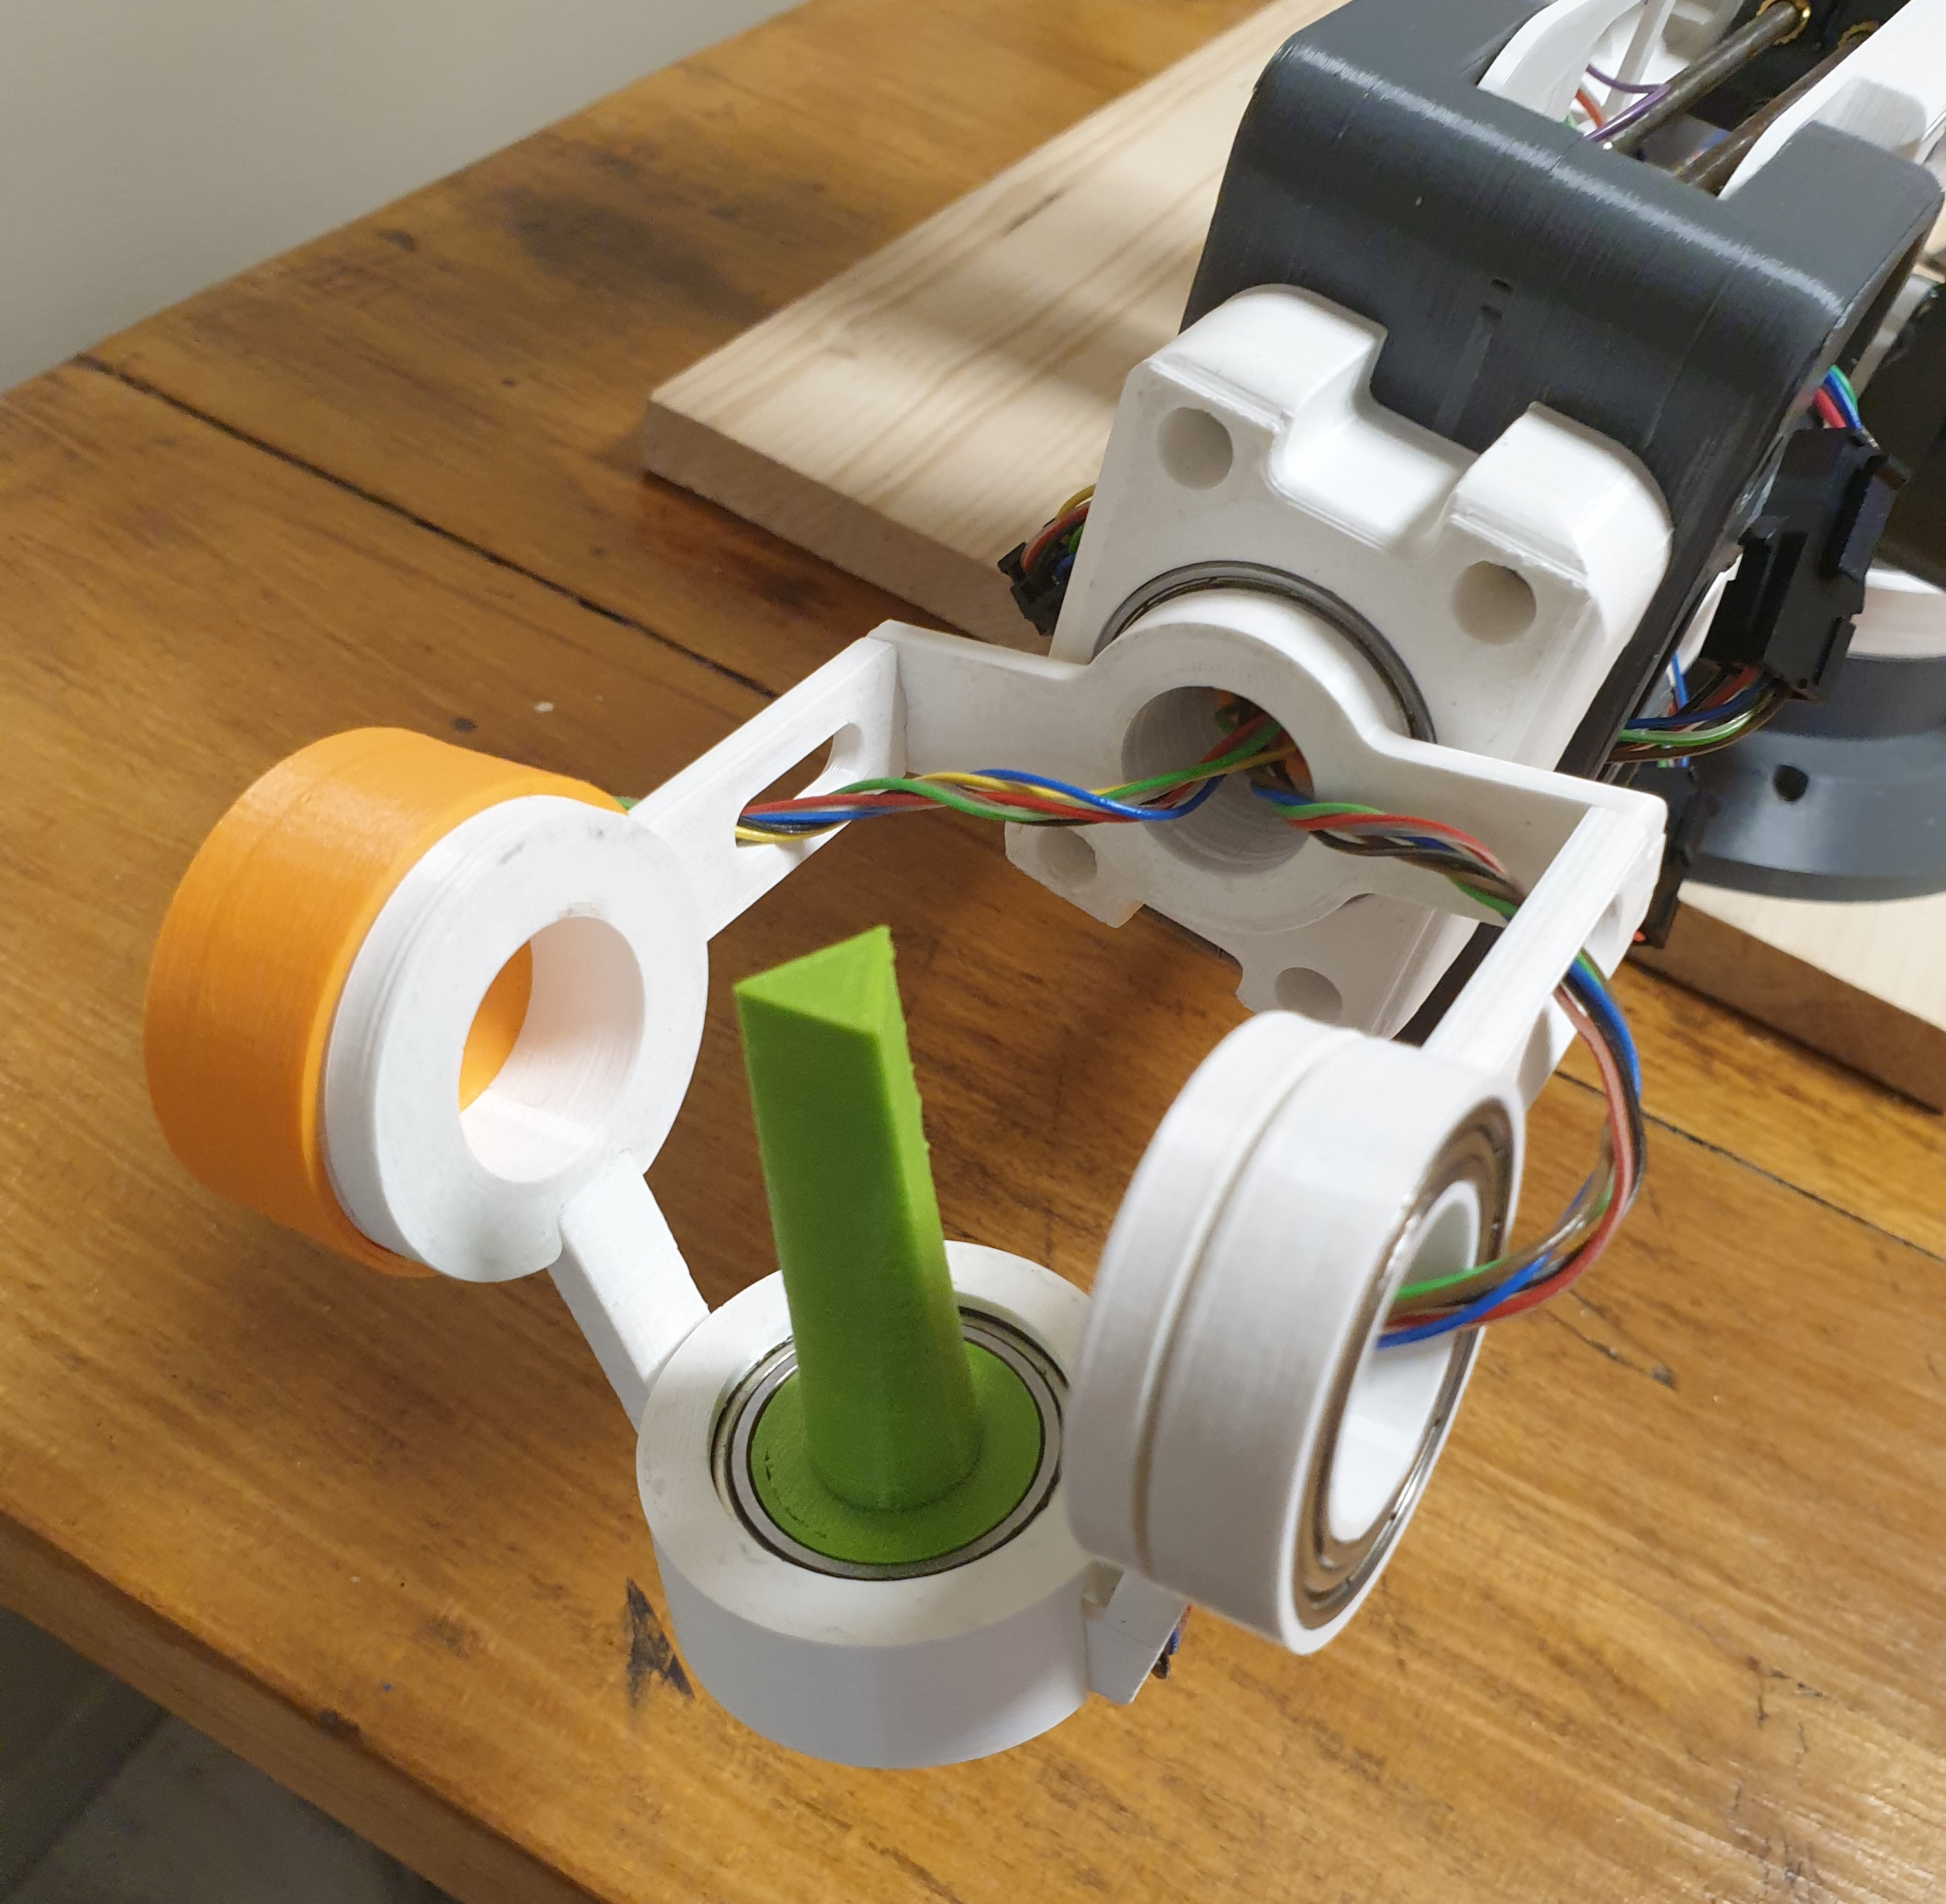
\includegraphics[width=70mm, keepaspectratio]{figures/Szumma/end_effektor}
\caption{Az end-effektor}
\label{fig:EE_fektor}
\end{figure}

A telemanipulátor tesztelése alatt, egy három csuklós end-effektort használtam. Ennek a kialakítása azt a cél szolgálja, hogy egyértelmű kinematikai láncán keresztül megteremtse mind a hat szabadsági fokot a felhasználó számára a vezérléshez. Egyértelmű TCP pontokat lehet vele felvenni és így ellenőrizni a kinematikai számítások és a későbbiekben bemutatásra kerülő robot kontroller működését.


\section{Kinematikai modell felépítése}

A TCP pont meghatározására több lehetőség van, de én a Denavit-Hartenberg(rövidítve DH) féle kinematikai felírást választottam. A módszerrel képes voltam meghatározni egy bázis koordináta rendszerhez viszonyítva a TCP pont hol található, illetve lehetőség van arra is hogy egy adott TCP pontot a rendszer milyen orientációban valósít meg. Ez a két irányú megközelítés a direkt és a inverz kinematikai felírás.

A direkt kinematikai felírása DH-alakkal úgy történik, hogy az abszolút nulla koordináta rendszerből csuklónként haladva azok orientációját rögzíteni kell. Ezeket a csukló orientációs együtthatókat a nevezzük DH-paramétereknek. A DH-alak felírásánál a koordináta rendszereket minden csuklóban úgy kell orientálni, hogy a $z$ tengely legyen a forgatási tengely, melynek meghatározása után már az $x,y$ tengelyek a jobb kéz szabály alapján adhatóak meg. Az $n$-edik koordináta rendszer az $n-1$ koordináta rendszeréhez viszonyított pozícióját a DH-paraméter összefoglaló táblázat rögzítik. A paraméterek között két szög forgatás, ami $x$ vagy $z$ tengely körül forgat és két eltolás, amik $x$ vagy $z$ tengely mentén mozgatnak. A $z$ tengely körüli forgatást $\theta$-ával, $x$ tengely körüli forgatást $\alpha$-ával, a $z$ tengely mentei eltolást $d$-vel és $x$ tengely menti eltolást $a$-val jelöltem a alkalmazása során. A paraméter megadási sorrend definiálva van. Sorrend szerint el végezhető transzformációk $\alpha$ -val lehet az $x$ körül forgatni, majd az $x$ tengelyen $a$-val eltolni. Ezt követően $\theta$-val a z tengely körül forgathatunk és $d$-vel ugyan ezen a tengelyen eltolhatunk. Ezt sorrendet minden körülmény között tartani kell.\cite{merat1987introduction}

\begin{figure}[!ht]
\centering
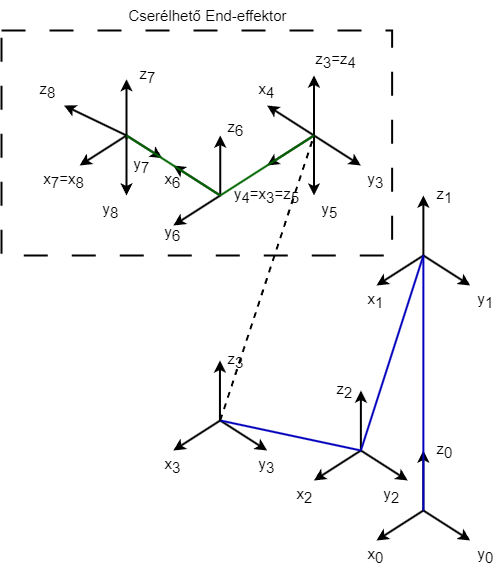
\includegraphics[width=90mm, keepaspectratio]{figures/Diagrammok/DH_feliras}
\caption{Diploma munka Denavit-Hartenberg felírás}
\label{fig:dip_dh}
\end{figure}

Az inverz kinematikát arra használtam, hogy egy ismert TCP pont és robotkarhoz tartozó DH transzformációs mátrix alapján megadjam, hogy a robotkar milyen orientációban tudja megvalósítani azt. A DH transzformációs paramétereket a Universal robot kontrollerébe a kontroller készítője programozta le, ezzel a kinematikai számítással nem foglalkoztam. Meg szeretném említeni azt, hogy az inverz kinematikai számítások nehézségét az adja, hogy több megoldása is lehet ha cél paraméter és a robotkar szabadsági fokainak száma azonos. TCP pontot ahogy említettem $x,y,z$ és $\alpha,\beta,\gamma$ paraméterekkel értelmezzük. A robotkar TCP pontja is képes mind a 6 paraméteren a kar fizikai limitáción belül szabadon mozogni. A gond ott keletkezik, hogy hat ismeretlen hat egyenlet megoldás esetén több megoldás is lehetségessé válik. Az ellentmondás feloldását csuklószög  limitekkel vagy közvetlen megoldással lehet orvosolni. \cite{merat1987introduction}\cite{merat1987introduction}

A következő táblázatban összefoglaltam az álltam használt DH paraméterek. Ezeket a paramétereket a későbbiekben az end-effektor változása esetén vagy bármilyen más változás esetén módosítani kell.\cite{merat1987introduction}

\begin{table}[!ht]
\centering
\caption{Denavit-Hartenberg paraméterek}
\begin{tabular}{|c|c|c|c|c|}
\hline
Csukló & $\alpha [rad]$ & a$[mm]$ & $\vartheta [rad]$  & d$[mm]$ \\ 
\hline
0  & 0  & 0 & $\vartheta_{1}$ & 290 \\ 
\hline
1  & 0  & $75+200*\sin(\vartheta_{2})$  & 0 & $-200*\cos(\vartheta_{2})+30$ \\ 
\hline
2  & 0  & $35+150*\cos(\vartheta_{3})$  & 0 & $150*\sin(\vartheta_{3})$ \\ 
\hline
3  & 0  & 0 & $-\frac{\pi}{2}$ & 0 \\ 
\hline
4  & $-\frac{\pi}{2}$  & 0 & $\vartheta_{4}$ & 95 \\ 
\hline
5  & $\frac{\pi}{2}$  & 0  & $\vartheta_{5}$ & 40 \\ 
\hline
6  & 0  & $50$ & $-\frac{\pi}{2}$ & 0 \\ 
\hline
7  & $-\frac{\pi}{2}$  & 0 & $\vartheta_{6}$ & 0  \\ 
\hline
\end{tabular}
\label{tab:DH_parameterek}
\end{table}

Két kiegészítő transzformációs mátrixot használok, amihez nem tartozik folyamatos szögelfordulás. Ezeknek a mátrixoknak a feladata $z$ tengely forgatása.\cite{merat1987introduction}

A dolgozatomban bemutatásra kerülő telemanipulátor kinematikai rendszerének koordináta transzformációs lépéseit a \ref{fig:dip_dh}.ábrán lehet látni. A későbbiekben szeretnék egy más típusú felírással is megpróbálkozni screw paraméter felírással. Ez a felírási módszer nagyon hasonlít a direkt kinematikai felíráshoz, azonban sokkal egyszerűbb. Nincs szükség a kinematikai tengelyek forgatásával foglalkozni.